\documentclass{article}

% Use the official NeurIPS 2026 style file. We compile in `preprint` mode for a
% readable draft; switch to `\usepackage{neurips_2026}` (default) for anonymous
% submission, or `\usepackage[final]{neurips_2026}` for camera-ready.
\usepackage[preprint]{neurips_2026}

\usepackage[utf8]{inputenc}
\usepackage[T1]{fontenc}
\usepackage{hyperref}
\usepackage{url}
\usepackage{booktabs}
\usepackage{amsfonts}
\usepackage{nicefrac}
\usepackage{microtype}
\usepackage{xcolor}
\usepackage{graphicx}
\usepackage{amsmath,amssymb,amsthm}
\usepackage{mathtools}

\theoremstyle{plain}
\newtheorem{theorem}{Theorem}
\newtheorem{lemma}[theorem]{Lemma}
\newtheorem{corollary}[theorem]{Corollary}
\newtheorem{proposition}[theorem]{Proposition}

\theoremstyle{definition}
\newtheorem{assumption}{Assumption}
\newtheorem{definition}[theorem]{Definition}

\theoremstyle{remark}
\newtheorem{remark}[theorem]{Remark}

\DeclareMathOperator{\Cov}{Cov}
\DeclareMathOperator{\tr}{tr}
\newcommand{\R}{\mathbb{R}}
\newcommand{\E}{\mathbb{E}}
\newcommand{\NN}{\mathcal{N}}
\newcommand{\Mem}{\mathrm{Mem}}
\newcommand{\hist}{\mathcal{H}}
\newcommand{\transcript}{\mathcal{T}}
\newcommand{\noised}{\widetilde{\Delta}}
\newcommand{\indep}{\perp\!\!\!\perp}

\title{Averaging Lowers Memorization in DP-FedAvg:\\
A Self-Contained Conditional-Mutual-Information Analysis}

\author{%
  Anonymous Author(s) \\
  Affiliation \\
  Address \\
  \texttt{email}
}

\begin{document}

\maketitle

\begin{abstract}
We study per-client memorization in differentially private federated averaging using the conditional mutual information measure introduced by \citet{Brown2021Memorization}. In one round of the protocol, each of \(K\) clients clips a local model update to Euclidean norm \(C\), and the server releases the average of the clipped updates with additive Gaussian noise of scale \(\sigma\). For every client \(k\) we prove \(I(X_k;\noised\mid P)\le C^2/(2K^2\sigma^2)\), where \(X_k\) denotes client \(k\)'s local dataset, \(\noised\) is the released averaged update, and \(P\) is the underlying data distribution. The proof applies a Gaussian-channel mutual information inequality directly to the per-client signal, without appealing to a differential-privacy guarantee as an intermediate step. We extend the bound to a \(T\)-round adaptive transcript \(\transcript\) via a telescoping chain-rule argument that correctly handles the dependences that past releases induce between \(X_k\) and the other clients' data, yielding \(I(X_k;\transcript\mid P)\le \sum_{t=0}^{T-1}C^2/(2K^2\sigma_t^2)\). The per-client bound is sharper, by a factor of \(K^2\), than both the whole-dataset bound \(I(X;\noised\mid P)\le C^2/(2\sigma^2)\) and the bound for the alternative protocol in which each client's clipped update is released individually with its own Gaussian noise of scale \(\sigma\), rather than averaged before the noise is added. We further refine the bound in two ways: a variance form replacing the worst-case clip \(C^2\) with the conditional update variance \(\tr\Cov(U_k\mid P)\), and a partial-participation analysis that yields a multiplicative \(q\) amplification when each client takes part in each round with probability \(q\), composing with the averaging factor \(1/K^2\) to give \(I(X_k;\transcript\mid P)\le qTC^2/(2K^2\sigma^2)\) over \(T\) rounds. Empirically, on a long-tailed Tiny-ImageNet benchmark with a Dirichlet client partition, the per-client train--test memorization gap collapses from approximately 75 percentage points at \(K=1\) to 15 points at \(K=10\). Averaging across clients before the noise is added---not the noise alone---is therefore the mechanism that suppresses individual-client memorization in this protocol.
\end{abstract}

\section{Introduction}\label{sec:intro}

In federated learning a central server coordinates training across \(K\) clients without collecting raw data. The canonical differentially private federated averaging algorithm (DP-FedAvg) of \citet{McMahan2018DPFedAvg} (see also \citealt{Geyer2017DPFedAvg}) proceeds round-by-round: each client returns a clipped update, the server averages the clipped updates, adds Gaussian noise, and broadcasts the new iterate. This is the federated counterpart of central differentially private stochastic gradient descent (DP-SGD; \citealt{Abadi2016DPSGD,DworkRoth2014Foundations}). We write \(\noised\) for the noised average released in a single round and \(\transcript=(\noised^{(0)},\dots,\noised^{(T-1)})\) for the full \(T\)-round transcript of releases (formal definitions in \S\ref{sec:setup} and \S\ref{sec:multi-setup}).

\citet{Brown2021Memorization} introduced an information-theoretic metric of memorization,
\[
\Mem(A;q)\;=\;I\bigl(X;\,A(X)\,\big|\,P\bigr),
\]
where \(P\sim q\) is a problem instance drawn from a meta-distribution \(q\), \(X\sim P^{\otimes n}\) is the dataset, and \(A(X)\) is the model. They showed that, on natural learning tasks, every sufficiently accurate algorithm must satisfy \(I(X;A(X)\mid P)=\Omega(nd)\). Their definition is precisely the conditional mutual information given the data distribution, not a per-record or worst-case quantity (cf.\ \citealp[Theorem~1.1, Section~1.1]{Brown2021Memorization}).

Translating this metric to the federated setting raises a natural question: in DP-FedAvg, how does the per-client memorization \(I(X_k; M\mid P)\) depend on \(K\), the clip bound \(C\), and the noise scale \(\sigma\)?

\paragraph{Contributions.} We give a fully explicit answer:
\begin{itemize}
\setlength\itemsep{2pt}
\item \textbf{One-round bound (Theorem~\ref{thm:one-round}).} For one round of DP-FedAvg, \(I(X_k;\noised \mid P)\le C^2/(2K^2\sigma^2)\). The proof uses only the Gaussian differential-entropy maximization inequality together with the data-processing inequality, and we make every conditional-independence step explicit.
\item \textbf{Multi-round bound (Theorem~\ref{thm:multi-round}).} For a \(T\)-round adaptive transcript \(\transcript = (\noised^{(0)},\dots,\noised^{(T-1)})\), \(I(X_k;\transcript\mid P)\le \sum_{t=0}^{T-1} C^2/(2K^2\sigma_t^2)\). Section~\ref{sec:gap} explains why the naive ``apply Theorem~\ref{thm:one-round} round-by-round and use the chain rule'' argument has a gap, and how a telescoping argument repairs it.
\item \textbf{Refinements (\S\ref{sec:refine}).} A variance-form bound replacing the worst-case clip \(C^2\) by the conditional update variance \(\tr\Cov(U_k\mid P)\), and a partial-participation analysis that yields a multiplicative \(q\) amplification when each client takes part in each round with probability \(q\), composing with the averaging factor \(1/K^2\) to give \(I(X_k;\transcript\mid P)\le qTC^2/(2K^2\sigma^2)\) over \(T\) rounds.
\item \textbf{Empirical confirmation (\S\ref{sec:experiments}).} On a long-tailed Tiny-ImageNet image-classification task with a Dirichlet client partition, we measure per-client and community-wise train/test accuracy as the number of clients grows. The empirical memorization gap collapses from roughly 75 percentage points at \(K=1\) to about 15 points at \(K=10\)---a monotone decrease consistent with the \(O(1/K^2)\) bound.
\item \textbf{Quantitative comparisons (\S\ref{sec:discuss}).} The per-client bound is a factor of \(K^2\) tighter than (i)~the whole-dataset bound \(I(X;\noised\mid P)\le C^2/(2\sigma^2)\), and (ii)~the per-client bound when each client's clipped + noised update is released without averaging. Averaging \emph{before} adding noise is therefore the active ingredient.
\end{itemize}

We deliberately avoid the chain ``Gaussian mechanism \(\Rightarrow\) \((\varepsilon,\delta)\)-differential privacy \(\Rightarrow\) per-record conditional mutual information (CMI)'' \citep[e.g.][]{BunSteinke2016,SteinkeUllman2017,Bassily2018ConcurrentCMI}. The direct route is shorter, gives explicit constants, and exposes \emph{why} averaging helps: each client's signal vector is scaled by \(1/K\) inside the average, so its squared energy by \(1/K^2\), and Lemma~\ref{lem:gauss-mi} converts squared signal energy into mutual information linearly.

\paragraph{Relation to prior work.} The mutual-information memorization measure dates to \citet{Bassily2018ConcurrentCMI,Russo2016ControllingBias}; \citet{Brown2021Memorization} sharpened it to the conditional form \(I(X;M\mid P)\) used here. DP-FedAvg analysis traditionally proceeds via \((\varepsilon,\delta)\)-differential privacy accounting (R\'enyi differential privacy or the moments accountant; see \citealt{Abadi2016DPSGD,KairouzMcMahan2021Practical}); we instead bound the CMI directly. Our proof for the multi-round case parallels classic adaptive composition arguments but operates on the CMI directly via a telescoping chain rule, which sidesteps the mismatch between marginal and conditional independence after seeing past releases.

\section{Preliminaries}\label{sec:prelim}

\subsection{Memorization in the sense of Brown et al.}\label{sec:mem-def}
We use the framework of \citet[\S1]{Brown2021Memorization}. Fix a meta-distribution \(q\) over problem instances \(P\), each itself a distribution on labeled examples. A learning algorithm \(A\) takes a dataset \(X\) of \(n\) i.i.d.\ examples from \(P\) and outputs \(M=A(X)\). The (conditional) memorization is
\begin{equation}\label{eq:mem-def}
\Mem(A;q) \;:=\; I\!\left(X;\,M\,\middle|\,P\right),
\end{equation}
computed in the joint model \(P\sim q,\;X\sim P^{\otimes n},\;M=A(X)\). Equation~\eqref{eq:mem-def} measures how much the model reduces uncertainty about the realized training set beyond what is implied by knowing the data distribution.

\subsection{Federated release model}\label{sec:setup}
We extend \citet{Brown2021Memorization} to a partitioned, \emph{potentially non-IID} dataset. There are \(K\ge 2\) clients, and we let the meta-distribution \(q\) sample a \emph{joint problem instance}
\[
P\;=\;(P_1,\dots,P_K),
\]
where each \(P_k\) is a distribution over labeled examples. Conditional on \(P\), client \(k\) draws its local dataset \(X_k\sim P_k^{\otimes n_k}\), independently across \(k\); we write \(X=(X_1,\dots,X_K)\) and \(X_{-k}\) for everything except client~\(k\). The original single-distribution setting of \citet{Brown2021Memorization} is the IID-FL special case in which \(q\) is supported on the diagonal \(P_1=\dots=P_K\); when we refer below to ``conditioning on \(P\)'' we mean conditioning on the entire tuple. Cross-client heterogeneity is therefore part of the model from the outset, not an extension. One round of DP-FedAvg, parametrized by the clip bound \(C>0\) and the noise scale \(\sigma>0\), proceeds as follows.
Given the current iterate \(\theta\), each client computes a (possibly randomized) raw update
\[
V_k \;=\; V_k(X_k,\theta,R_k) \;\in\; \R^d,
\]
using fresh client randomness \(R_k\), and clips it to the ball of radius \(C\):
\begin{equation}\label{eq:clip}
U_k \;:=\; \mathrm{clip}_C(V_k) \;=\; V_k \cdot \min\!\Bigl\{1,\ \frac{C}{\|V_k\|_2}\Bigr\}, \qquad\text{so } \|U_k\|_2 \le C \text{ by construction.}
\end{equation}
The server averages the clipped updates and adds Gaussian noise:
\begin{equation}\label{eq:release}
    \noised \;:=\; \frac{1}{K}\sum_{k=1}^{K} U_k \;+\; Z, \qquad Z\sim\NN\!\left(0,\sigma^2 I_d\right),
\end{equation}
with \(Z\) drawn independently of all data and client randomness. The bound \(\|U_k\|_2\le C\) is part of the algorithm specification, not a hypothesis on \(V_k\); the analysis goes through for any choice of raw update map \(V_k\).
We make one assumption on the data-generating process:

\begin{assumption}[Conditional independence given the joint instance]\label{ass:indep}
Conditional on \(P=(P_1,\dots,P_K)\), the client datasets \(X_1,\dots,X_K\) are mutually independent, with \(X_k\sim P_k^{\otimes n_k}\) drawn from the \(k\)-th component. The client randomness \((R_1,\dots,R_K)\) is mutually independent and independent of \((X_1,\dots,X_K)\) and of \(P\). The server noise \(Z\) is drawn fresh, independent of \((X,R_1,\dots,R_K,P)\).
\end{assumption}

Assumption~\ref{ass:indep} generalizes the Brown et al.\ generative model from a single distribution to a tuple of per-client distributions, and is the independence model used implicitly in standard FL analyses (e.g., \citealt{Bornstein2022SWIFT}). The IID-FL special case (\(P_1=\dots=P_K\)) is recovered when \(q\) is concentrated on the diagonal; the non-IID case is the generic one and is what we have in mind throughout. The assumption restricts only the joint generation of client datasets given \(P\); it does \emph{not} restrict the per-client distributions \(P_k\) themselves, which may have arbitrarily different supports, label balance, or label-conditional structure across \(k\). All of the per-client memorization bounds below condition on the full tuple \(P\), so the inter-client heterogeneity is integrated into the conditioning rather than treated as adversarial perturbation.

\section{A direct Gaussian-channel mutual-information bound}\label{sec:lemma}

The only information-theoretic ingredient we need is the following standard bound; see, e.g., \citet[\S9]{CoverThomas2006}.

\begin{lemma}[Bounded-energy MI through additive Gaussian noise]\label{lem:gauss-mi}
Let \(S\) be an \(\R^d\)-valued random variable with \(\E\|S\|_2^2<\infty\), and let \(Z\sim\NN(0,\sigma^2 I_d)\) be independent of \(S\). Then
\begin{equation}\label{eq:gauss-mi}
I(S;\,S+Z) \;\le\; \tfrac{1}{2}\log\det\!\Bigl(I_d+\tfrac{1}{\sigma^2}\Cov(S)\Bigr)
\;\le\; \frac{1}{2\sigma^2}\,\tr\Cov(S) \;=\; \frac{1}{2\sigma^2}\,\E\|S-\E S\|_2^2 \;\le\; \frac{1}{2\sigma^2}\,\E\|S\|_2^2.
\end{equation}
Moreover, for any random variable \(W\) such that the joint pair \((S,W)\) is independent of \(Z\), the same chain holds conditionally; in particular,
\begin{equation}\label{eq:gauss-mi-cond}
I(S;\,S+Z\mid W) \;\le\; \frac{1}{2\sigma^2}\,\E\!\bigl[\,\|S-\E[S\mid W]\|_2^2\,\bigr] \;\le\; \frac{1}{2\sigma^2}\,\E\|S\|_2^2.
\end{equation}
\end{lemma}

\begin{proof}
We use \(I(S;S+Z) = h(S+Z) - h(S+Z\mid S) = h(S+Z) - h(Z)\), since conditional on \(S\) the random variable \(S+Z\) has the same density as \(Z\). Among all distributions on \(\R^d\) with a fixed second-moment matrix, the Gaussian maximizes differential entropy \citep[Theorem 8.6.5]{CoverThomas2006}, so
\[
h(S+Z)\;\le\;\tfrac{1}{2}\log\!\left((2\pi e)^d \det\!\bigl(\Cov(S)+\sigma^2 I_d\bigr)\right),
\]
where we used \(\Cov(S+Z)=\Cov(S)+\sigma^2 I_d\) by independence of \(S\) and \(Z\). Combining with \(h(Z)=\tfrac{1}{2}\log\!\bigl((2\pi e)^d \det(\sigma^2 I_d)\bigr)\) yields
\[
I(S;S+Z)\;\le\;\tfrac{1}{2}\log\det\!\Bigl(I_d+\tfrac{1}{\sigma^2}\Cov(S)\Bigr).
\]
The eigenvalue inequality \(\log(1+\lambda)\le\lambda\) gives \(\log\det(I_d+M)\le \tr(M)\) for PSD \(M\), so
\[
I(S;S+Z)\;\le\;\tfrac{1}{2\sigma^2}\,\tr\Cov(S)\;=\;\tfrac{1}{2\sigma^2}\,\E\|S-\E S\|_2^2.
\]
The final inequality in~\eqref{eq:gauss-mi} is \(\E\|S-\E S\|_2^2 = \E\|S\|^2-\|\E S\|^2 \le \E\|S\|^2\).

For the conditional version, condition on \(W=w\). Since \(Z\indep(S,W)\), conditional on \(W=w\) the noise \(Z\) is still \(\NN(0,\sigma^2 I_d)\) and independent of \(S\mid W=w\). Apply~\eqref{eq:gauss-mi} to the conditional distribution and integrate against \(P_W\) using the tower property and Jensen's inequality on the variance to obtain~\eqref{eq:gauss-mi-cond}.
\end{proof}

\begin{remark}[Tightness of the bounds in Lemma~\ref{lem:gauss-mi}]\label{rem:variance}
The first inequality in~\eqref{eq:gauss-mi} is the Gaussian channel capacity expression and is \emph{tight}: equality holds iff \(S\) is Gaussian, in which case \(S+Z\) is also Gaussian and the differential-entropy maximization step is exact. The second inequality, \(\log\det(I+M)\le\tr(M)\), uses \(\log(1+\lambda)\le\lambda\) eigenvalue-wise and is loose unless the eigenvalues of \(\Cov(S)/\sigma^2\) are all small (low-SNR regime); when \(\Cov(S) = c\cdot I_d\) with \(c\ll\sigma^2\), the gap is \(O(c^2/\sigma^4)\) per coordinate. The variance form \(\tfrac{1}{2\sigma^2}\E\|S-\E S\|^2\) is sharper than the often-quoted \(\tfrac{1}{2\sigma^2}\E\|S\|^2\) by \(\|\E S\|^2/(2\sigma^2)\); both can be much smaller than the worst-case clip when client updates concentrate.
\end{remark}

\section{One-round per-client memorization bound}\label{sec:one-round}

\begin{theorem}[One-round]\label{thm:one-round}
Fix \(C>0\) and \(\sigma>0\) and let \(\noised\) be the one-round DP-FedAvg release defined by~\eqref{eq:clip}--\eqref{eq:release}. Under Assumption~\ref{ass:indep}, for every \(k\in\{1,\dots,K\}\),
\begin{equation}\label{eq:one-round}
I(X_k;\,\noised \mid P) \;\le\; \frac{C^2}{2 K^2 \sigma^2}.
\end{equation}
\end{theorem}

\begin{proof}
Fix \(k\). Decompose
\[
\noised \;=\; \tfrac{1}{K}U_k \;+\; W_k \;+\; Z, \qquad W_k \;:=\; \tfrac{1}{K}\sum_{j\ne k}U_j.
\]

\textbf{Step 1: \(X_k\indep W_k\mid P\).}
By Assumption~\ref{ass:indep}, conditional on \(P\) the pair \((X_k,R_k)\) is independent of \((X_{-k},R_{-k})\); since \(U_k=\mathrm{clip}_C(V_k(X_k,\theta,R_k))\) is a measurable function of \((X_k,R_k,\theta)\) and \(W_k\) is a measurable function of \((X_{-k},R_{-k},\theta)\) (with \(\theta\) constant in this round), this gives \((X_k,U_k)\indep W_k\mid P\). Also, \(Z\indep(X,R_1,\dots,R_K,P)\), so \(Z\indep(X_k,U_k,W_k)\mid P\) as well.

\textbf{Step 2: a chain-rule sandwich.}
Apply the chain rule for conditional MI two ways:
\begin{align*}
I(X_k;\,\noised,W_k\mid P)
&\;=\;I(X_k;W_k\mid P)+I(X_k;\noised\mid P,W_k)\\
&\;=\;0+I(X_k;\noised\mid P,W_k)
&\text{(using Step 1)}\\
I(X_k;\,\noised,W_k\mid P)
&\;=\;I(X_k;\noised\mid P)+I(X_k;W_k\mid P,\noised).
\end{align*}
Since \(I(X_k;W_k\mid P,\noised)\ge 0\), the two equalities give
\begin{equation}\label{eq:remove-W}
I(X_k;\noised\mid P) \;\le\; I(X_k;\noised\mid P,W_k).
\end{equation}

\textbf{Step 3: subtract the known shift.}
Conditional on \((P,W_k)\), \(W_k\) is a fixed quantity, so \(\noised - W_k = \tfrac{1}{K}U_k+Z\) is a measurable bijection of \(\noised\). Hence
\begin{equation}\label{eq:bijection-step}
I(X_k;\noised\mid P,W_k) \;=\; I\!\left(X_k;\,\tfrac{1}{K}U_k+Z\,\middle|\,P,W_k\right).
\end{equation}
By Step~1, \(W_k\indep(X_k,U_k,Z)\mid P\), so conditioning further on \(W_k\) does not change the joint distribution of \((X_k,\tfrac{1}{K}U_k+Z)\) given \(P\):
\begin{equation}\label{eq:condition-out-W}
I\!\left(X_k;\,\tfrac{1}{K}U_k+Z\,\middle|\,P,W_k\right) \;=\; I\!\left(X_k;\,\tfrac{1}{K}U_k+Z\,\middle|\,P\right).
\end{equation}

\textbf{Step 4: data processing and Gaussian channel.}
Conditional on \(P\), we have the Markov chain \(X_k\to U_k\to \tfrac{1}{K}U_k+Z\) (the second arrow uses fresh \(R_k\) and \(Z\), independent of everything else given \(P\)). Conditional data processing gives
\begin{equation}\label{eq:dpi}
I\!\left(X_k;\,\tfrac{1}{K}U_k+Z\,\middle|\,P\right)\;\le\;I\!\left(U_k;\,\tfrac{1}{K}U_k+Z\,\middle|\,P\right)\;=\;I\!\left(\tfrac{1}{K}U_k;\,\tfrac{1}{K}U_k+Z\,\middle|\,P\right),
\end{equation}
using that multiplication by \(K\) is a bijection. Apply the conditional Gaussian-channel bound~\eqref{eq:gauss-mi-cond} with \(S=\tfrac{1}{K}U_k\) and conditioning variable \(P\) (recalling that \(Z\indep(S,P)\)):
\begin{equation}\label{eq:lemma1-step}
I\!\left(\tfrac{1}{K}U_k;\,\tfrac{1}{K}U_k+Z\,\middle|\,P\right)\;\le\;\frac{1}{2\sigma^2}\,\E\!\left[\big\|\tfrac{1}{K}U_k\big\|_2^2\right]\;\le\;\frac{C^2}{2K^2\sigma^2},
\end{equation}
where the last inequality uses \(\|U_k\|_2\le C\) by construction~\eqref{eq:clip}. Chaining \eqref{eq:remove-W}--\eqref{eq:lemma1-step} yields~\eqref{eq:one-round}.
\end{proof}

\begin{remark}[Sharpening via variance]
Replacing the last inequality in~\eqref{eq:lemma1-step} by \(\tfrac{1}{2\sigma^2}\E\|\tfrac{1}{K}U_k-\E[\tfrac{1}{K}U_k\mid P]\|_2^2\) gives a strictly sharper bound when client updates concentrate (Remark~\ref{rem:variance}); the form~\eqref{eq:one-round} uses only the worst-case clip.
\end{remark}

\section{Multi-round transcript bound}\label{sec:multi-round}

\subsection{Multi-round release model}\label{sec:multi-setup}
For \(t=0,1,\dots,T-1\), at round \(t\) the server holds an iterate \(\theta^{(t)}\) (a deterministic function of past releases\footnote{If the server uses additional randomness to update \(\theta^{(t)}\), independent of all data, simply augment the conditioning by that randomness; the proof is unchanged.}). Each client \(k\) draws fresh \(R_k^{(t)}\), produces a raw update \(V_k^{(t)}=V_k^{(t)}(X_k,\theta^{(t)},R_k^{(t)})\), and clips it: \(U_k^{(t)} := \mathrm{clip}_C(V_k^{(t)})\), so \(\|U_k^{(t)}\|_2\le C\) by construction. The server releases
\begin{equation}\label{eq:release-t}
\noised^{(t)} \;:=\; \frac{1}{K}\sum_{k=1}^{K}U_k^{(t)} \;+\; Z^{(t)}, \qquad Z^{(t)}\sim\NN\!\bigl(0,\sigma_t^2 I_d\bigr),
\end{equation}
with \(\{Z^{(t)}\}_t\) and \(\{R_k^{(t)}\}_{k,t}\) mutually independent and independent of \((X,P)\). Let \(\transcript:=(\noised^{(0)},\dots,\noised^{(T-1)})\) and \(\hist^{(t)}:=(\noised^{(0)},\dots,\noised^{(t-1)})\), with \(\hist^{(0)}=\varnothing\).

\subsection{Why the one-round argument does not directly compose}\label{sec:gap}
A natural attempt is the chain rule
\(I(X_k;\transcript\mid P) = \sum_t I(X_k;\noised^{(t)}\mid P,\hist^{(t)})\) followed by the one-round proof at each \(t\), with the conditioning augmented by \(\hist^{(t)}\). \emph{This argument has a gap.}
The one-round proof crucially used \(X_k\indep W_k\mid P\) (Step~1 of Theorem~\ref{thm:one-round}). After conditioning on \(\hist^{(t)}\), this fails: observing \(\noised^{(0)},\dots,\noised^{(t-1)}\) couples \(X_k\) with \(X_{-k}\) (an explaining-away effect), so in general
\(X_k\not\indep W_k^{(t)}\mid P,\hist^{(t)}\). The chain-rule sandwich~\eqref{eq:remove-W} is no longer available with \(W_k^{(t)}\) playing the role of \(W_k\). We repair the argument by conditioning on the \emph{full} \(X_{-k}\) instead of on \(W_k^{(t)}\), exploiting that \(X_k\indep X_{-k}\mid P\) marginally.

\subsection{Theorem and proof}

\begin{theorem}[Multi-round transcript memorization]\label{thm:multi-round}
Fix \(C>0\) and a noise schedule \(\{\sigma_t\}_{t=0}^{T-1}\), and let \(\transcript\) be the \(T\)-round DP-FedAvg transcript defined by~\eqref{eq:release-t}. Under Assumption~\ref{ass:indep}, with \((R_k^{(t)})_{k,t}\) and \((Z^{(t)})_t\) mutually independent fresh randomness, for every \(k\in\{1,\dots,K\}\),
\begin{equation}\label{eq:multi-round}
I(X_k;\transcript\mid P) \;\le\; \sum_{t=0}^{T-1} \frac{C^2}{2K^2\sigma_t^2}.
\end{equation}
In particular, with \(\sigma_t\equiv\sigma\), \(I(X_k;\transcript\mid P)\le \nicefrac{TC^2}{(2K^2\sigma^2)}\). Moreover, for any deterministic post-processing of the transcript---in particular, for the final iterate \(\theta^{(T)}\), which is a deterministic function of \(\transcript\)---the data-processing inequality yields
\begin{equation}\label{eq:final-iterate}
    I\!\left(X_k;\,\theta^{(T)}\,\middle|\,P\right) \;\le\; I(X_k;\transcript\mid P) \;\le\; \sum_{t=0}^{T-1}\frac{C^2}{2K^2\sigma_t^2}.
\end{equation}
\end{theorem}

\begin{proof}
\textbf{Step A: lift the conditioning to \(X_{-k}\).}
Mutual information is monotone under augmenting the second argument: for any random variables \(A,B,C,D\), the chain rule \(I(A;B,C\mid D) = I(A;B\mid D) + I(A;C\mid D,B)\) and non-negativity of conditional MI give \(I(A;B\mid D)\le I(A;B,C\mid D)\). Apply this with \(A=X_k\), \(B=\transcript\), \(C=X_{-k}\), \(D=P\), then expand the right-hand side by the chain rule the other way and use \(I(X_k;X_{-k}\mid P)=0\) (Assumption~\ref{ass:indep}):
\begin{align}
I(X_k;\transcript\mid P)
&\;\le\;I(X_k;\transcript,X_{-k}\mid P)\notag\\
&\;=\;I(X_k;X_{-k}\mid P)+I(X_k;\transcript\mid P,X_{-k})\notag\\
&\;=\;I(X_k;\transcript\mid P,X_{-k}). \label{eq:lift}
\end{align}

\textbf{Step B: chain-rule expansion of the lifted MI.}
Applying the chain rule for conditional MI to \(\transcript=(\noised^{(0)},\dots,\noised^{(T-1)})\) given \((P,X_{-k})\):
\begin{equation}\label{eq:chain-T}
I(X_k;\transcript\mid P,X_{-k}) \;=\; \sum_{t=0}^{T-1} I\!\left(X_k;\,\noised^{(t)}\,\middle|\,P,X_{-k},\hist^{(t)}\right).
\end{equation}

\textbf{Step C: bound each round under full \(X_{-k}\) conditioning.}
Fix a round \(t\) and condition on \(\mathcal C_t := (P,X_{-k},\hist^{(t)})\). The random variable
\[
W_k^{(t)} \;=\; \tfrac{1}{K}\sum_{j\ne k}U_j^{(t)}\!\left(X_j,\theta^{(t)},R_j^{(t)}\right)
\]
is, in general, a measurable function of \((X_{-k},\theta^{(t)},R_{-k}^{(t)})\), where \(R_{-k}^{(t)}:=\{R_j^{(t)}\}_{j\ne k}\). Conditioning on \(\mathcal C_t\) fixes \(X_{-k}\), and \(\theta^{(t)}\) is a deterministic function of \(\hist^{(t)}\subseteq\mathcal C_t\) and is hence also fixed. Therefore, under the conditional measure \(P(\,\cdot\mid\mathcal C_t)\), the only stochastic input to \(W_k^{(t)}\) is \(R_{-k}^{(t)}\), which is fresh randomness independent of \((X_k,R_k^{(t)},Z^{(t)})\). Consequently:
\begin{equation}\label{eq:multi-indep}
W_k^{(t)} \indep X_k \mid \mathcal C_t, \qquad Z^{(t)}\indep(X_k,U_k^{(t)},W_k^{(t)})\mid \mathcal C_t.
\end{equation}
Now repeat Steps 2--4 of the one-round proof with conditioning variable \(\mathcal C_t\) in place of \(P\):
\begin{align*}
I(X_k;\noised^{(t)}\mid\mathcal C_t)
&\;\stackrel{(*)}{\le}\; I(X_k;\noised^{(t)}\mid\mathcal C_t,W_k^{(t)})\\
&\;=\;I\!\left(X_k;\,\tfrac{1}{K}U_k^{(t)}+Z^{(t)}\,\middle|\,\mathcal C_t,W_k^{(t)}\right)\\
&\;=\;I\!\left(X_k;\,\tfrac{1}{K}U_k^{(t)}+Z^{(t)}\,\middle|\,\mathcal C_t\right)\\
&\;\le\; I\!\left(\tfrac{1}{K}U_k^{(t)};\,\tfrac{1}{K}U_k^{(t)}+Z^{(t)}\,\middle|\,\mathcal C_t\right) \\
&\;\le\;\frac{1}{2\sigma_t^2}\E\!\left[\bigl\|\tfrac{1}{K}U_k^{(t)}\bigr\|_2^2\right]
\;\le\;\frac{C^2}{2K^2\sigma_t^2},
\end{align*}
where \((*)\) uses~\eqref{eq:multi-indep} with the same chain-rule sandwich as~\eqref{eq:remove-W}; the second equality uses \(W_k^{(t)}\indep(X_k,U_k^{(t)},Z^{(t)})\mid\mathcal C_t\) (which is the conjunction of~\eqref{eq:multi-indep} and the freshness of \(Z^{(t)}\)); the data-processing step uses the Markov chain \(X_k\to U_k^{(t)}\to \tfrac{1}{K}U_k^{(t)}+Z^{(t)}\) given \(\mathcal C_t\); and the last inequality is Lemma~\ref{lem:gauss-mi} applied conditionally together with \(\|U_k^{(t)}\|_2\le C\) by construction.

\textbf{Step D: combine.}
Plugging Step~C into~\eqref{eq:chain-T} and combining with~\eqref{eq:lift} gives~\eqref{eq:multi-round}. The post-processing claim is the data-processing inequality applied to the deterministic map \(\transcript\mapsto\theta^{(T)}\).
\end{proof}

\begin{remark}[Why the lift to \(X_{-k}\) is free]
Step~A uses only \(I(X_k;X_{-k}\mid P)=0\), the cleanest consequence of Assumption~\ref{ass:indep}. Lifting the conditioning to \(X_{-k}\) (rather than to \(W_k^{(t)}\) round-by-round) sidesteps the explaining-away dependence created by past releases entirely.
\end{remark}

\section{Refinements: variance form and partial participation}\label{sec:refine}

The proofs of Theorems~\ref{thm:one-round} and~\ref{thm:multi-round} discard two pieces of structure that are present in real DP-FedAvg deployments and that tighten the bound substantively. First, the worst-case clip bound \(\|U_k^{(t)}\|_2\le C\) replaces \(\E\|S-\E S\|_2^2\) in Lemma~\ref{lem:gauss-mi}, which is loose whenever client updates concentrate around a population mean. Second, deployed DP-FedAvg almost never has every client participate in every round; instead, an independent random subset of clients is selected per round. We now give a single combined refinement that captures both effects.

\subsection{Variance-form bound (full participation)}

\begin{theorem}[Variance-form one-round bound]\label{thm:var-one-round}
Under the conditions of Theorem~\ref{thm:one-round},
\begin{equation}\label{eq:var-one-round}
I(X_k;\noised\mid P)\;\le\;\frac{\E\!\left[\tr\Cov(U_k\mid P)\right]}{2K^2\sigma^2}\;\le\;\frac{C^2}{2K^2\sigma^2},
\end{equation}
where \(\Cov(U_k\mid P)\) denotes the covariance matrix of \(U_k\) under the conditional distribution given \(P\), and the outer expectation is over \(P\sim q\).
\end{theorem}

\begin{proof}
Replace the last inequality \(\E\|\tfrac{1}{K}U_k\|_2^2\le C^2/K^2\) in~\eqref{eq:lemma1-step} with the conditional version of Lemma~\ref{lem:gauss-mi} stated as~\eqref{eq:gauss-mi-cond}, applied with \(S=\tfrac{1}{K}U_k\) and conditioning variable \(P\):
\[
I\!\left(\tfrac{1}{K}U_k;\,\tfrac{1}{K}U_k+Z\,\middle|\,P\right)\;\le\;\frac{1}{2\sigma^2}\,\E\!\left[\bigl\|\tfrac{1}{K}U_k-\E[\tfrac{1}{K}U_k\mid P]\bigr\|_2^2\right]\;=\;\frac{\E[\tr\Cov(U_k\mid P)]}{2K^2\sigma^2}.
\]
The remaining inequality follows from \(\tr\Cov(U_k\mid P)\le\E[\|U_k\|_2^2\mid P]\le C^2\).
\end{proof}

\subsection{Combined: variance form under partial participation}

We now extend the multi-round model of \S\ref{sec:multi-setup} to allow partial participation. For each round \(t\) and each client \(k\), let \(A_k^{(t)}\sim\mathrm{Bernoulli}(q)\) with \(q\in(0,1]\) be a fresh participation indicator, drawn independently across \(k\) and \(t\) and independently of all data and other algorithmic randomness. The released update is
\begin{equation}\label{eq:release-t-pp}
\noised^{(t)} \;:=\; \frac{1}{K}\sum_{k=1}^{K} A_k^{(t)}\,U_k^{(t)} \;+\; Z^{(t)},\qquad Z^{(t)}\sim\NN(0,\sigma_t^2 I_d).
\end{equation}
We refer to this as DP-FedAvg with Bernoulli participation rate \(q\); \(q=1\) is the full-participation model of~\eqref{eq:release-t}.

For each \((k,t)\), define the conditional update variance
\begin{equation}\label{eq:vkt}
v_k^{(t)} \;:=\; \E\!\left[\tr\Cov\!\left(U_k^{(t)}\,\Big|\,P,X_{-k},\hist^{(t)}\right)\right].
\end{equation}
Since \(\|U_k^{(t)}\|_2\le C\) by construction, we have \(v_k^{(t)}\le C^2\) for every \(k,t\).

\begin{theorem}[Variance-form transcript bound under partial participation]\label{thm:var-pp}
Under Assumption~\ref{ass:indep} extended by independent Bernoulli participation indicators as above, with \((R_k^{(t)})_{k,t}\), \((Z^{(t)})_t\), and \((A_k^{(t)})_{k,t}\) mutually independent fresh randomness independent of \((X,P)\),
\begin{equation}\label{eq:var-pp}
I(X_k;\transcript\mid P)\;\le\;\sum_{t=0}^{T-1}\frac{q\,v_k^{(t)}}{2K^2\sigma_t^2}\;\le\;q\sum_{t=0}^{T-1}\frac{C^2}{2K^2\sigma_t^2}.
\end{equation}
The same bound applies, by data processing, to any deterministic post-processing of \(\transcript\), e.g.\ the final iterate \(\theta^{(T)}\).
\end{theorem}

\begin{proof}
Steps~A and~B of the proof of Theorem~\ref{thm:multi-round} are unchanged: \(I(X_k;\transcript\mid P)\le I(X_k;\transcript\mid P,X_{-k})=\sum_t I(X_k;\noised^{(t)}\mid P,X_{-k},\hist^{(t)})\). We modify Step~C.

\textbf{Step C': augmented conditioning by the participation pattern.}
Fix a round \(t\) and condition on \(\mathcal C_t:=(P,X_{-k},\hist^{(t)})\). Let \(A^{(t)}:=(A_1^{(t)},\dots,A_K^{(t)})\) denote the round-\(t\) participation pattern. Since \(A^{(t)}\) is fresh randomness independent of all data, \(A^{(t)}\indep X_k\mid\mathcal C_t\); equivalently \(I(X_k;A^{(t)}\mid\mathcal C_t)=0\). Applying the chain-rule sandwich identical to~\eqref{eq:remove-W} (with \(A^{(t)}\) in the role of \(W_k\)),
\begin{equation}\label{eq:augment-A}
I(X_k;\noised^{(t)}\mid\mathcal C_t)\;\le\;I(X_k;\noised^{(t)}\mid\mathcal C_t,A^{(t)}).
\end{equation}

\textbf{Step C'': bound conditional on the realized pattern.}
Decompose \(\noised^{(t)}=(1/K)\,A_k^{(t)}\,U_k^{(t)}+\widetilde W_k^{(t)}+Z^{(t)}\) where \(\widetilde W_k^{(t)}:=(1/K)\sum_{j\ne k}A_j^{(t)}U_j^{(t)}\). Conditional on \((\mathcal C_t,A^{(t)})\), the quantities \(X_{-k}\), \(\theta^{(t)}\), and \(A^{(t)}\) are fixed; \(\widetilde W_k^{(t)}\) is a measurable function of the fresh randomness \(R_{-k}^{(t)}\) only, and is therefore independent of \((X_k,U_k^{(t)},Z^{(t)})\) given \((\mathcal C_t,A^{(t)})\).

\emph{Subcase \(A_k^{(t)}=0\).} Then \((1/K)\,A_k^{(t)}\,U_k^{(t)}=0\) and \(\noised^{(t)}=\widetilde W_k^{(t)}+Z^{(t)}\) is a measurable function of objects conditionally independent of \(X_k\); hence
\(I(X_k;\noised^{(t)}\mid\mathcal C_t,A^{(t)},A_k^{(t)}=0)=0\).

\emph{Subcase \(A_k^{(t)}=1\).} The signal is \((1/K)U_k^{(t)}+\widetilde W_k^{(t)}+Z^{(t)}\), to which Steps~2--4 of the proof of Theorem~\ref{thm:one-round} apply with conditioning variable \((\mathcal C_t,A^{(t)})\) replacing \(P\):
\[
I\!\left(X_k;\,\noised^{(t)}\,\middle|\,\mathcal C_t,A^{(t)},A_k^{(t)}=1\right)\;\le\;\frac{\tr\Cov\!\left(U_k^{(t)}\mid\mathcal C_t,A^{(t)}\right)}{2K^2\sigma_t^2}\,.
\]
Since \(U_k^{(t)}=U_k^{(t)}(X_k,\theta^{(t)},R_k^{(t)})\) does not depend on \(A^{(t)}\), and \(A^{(t)}\) is independent of \((X_k,R_k^{(t)})\) given \(\mathcal C_t\), the conditional covariance is unchanged by augmenting with \(A^{(t)}\):
\[
\Cov\!\left(U_k^{(t)}\mid\mathcal C_t,A^{(t)}\right)\;=\;\Cov\!\left(U_k^{(t)}\mid\mathcal C_t\right).
\]

\textbf{Step C''': marginalize over \(A_k^{(t)}\) and over \(\mathcal C_t\).}
Combining the two subcases and using \(\Pr[A_k^{(t)}=1]=q\),
\[
I(X_k;\noised^{(t)}\mid\mathcal C_t,A^{(t)})\;\le\;q\cdot\frac{\tr\Cov(U_k^{(t)}\mid\mathcal C_t)}{2K^2\sigma_t^2}.
\]
Substituting into~\eqref{eq:augment-A} and taking expectation over \(\mathcal C_t\),
\[
I(X_k;\noised^{(t)}\mid P,X_{-k},\hist^{(t)})\;\le\;\frac{q\,v_k^{(t)}}{2K^2\sigma_t^2}.
\]
Summing over \(t\) and combining with Steps~A, B yields~\eqref{eq:var-pp}.
\end{proof}

\begin{remark}[Special cases]\label{rem:special}
Setting \(q=1\) in Theorem~\ref{thm:var-pp} recovers a variance-form strengthening of Theorem~\ref{thm:multi-round}: \(I(X_k;\transcript\mid P)\le\sum_t v_k^{(t)}/(2K^2\sigma_t^2)\). Setting \(\sigma_t\equiv\sigma\) and \(v_k^{(t)}\le C^2\) gives the headline bound \(I(X_k;\transcript\mid P)\le qTC^2/(2K^2\sigma^2)\): partial participation contributes a multiplicative factor \(q\) on top of the averaging factor \(1/K^2\). The two amplifications combine cleanly because the participation indicator \(A_k^{(t)}\) is independent of the data and acts as an independent zero-out of the per-client signal.
\end{remark}

\begin{remark}[Cohort sampling without replacement]\label{rem:cohort}
The same proof handles the common ``sample a cohort of \(m\) clients without replacement at each round'' protocol, where client \(k\) participates with marginal probability \(m/K\). The bound becomes \(I(X_k;\transcript\mid P)\le\sum_t (m/K)\,v_k^{(t)}/(2K^2\sigma_t^2)\); the fact that participation indicators \(A_k^{(t)}\) are now negatively correlated across \(k\) at fixed \(t\) does not affect the argument, which only used the marginal independence \(A_k^{(t)}\indep X_k\mid\mathcal C_t\).
\end{remark}

\begin{remark}[When does the variance form help?]\label{rem:variance-help}
Whenever client updates concentrate around a conditional mean given \(P\)---a regime that is empirically common when the optimization landscape has a stable population minimizer---we have \(\tr\Cov(U_k\mid P)\ll C^2\), and~\eqref{eq:var-pp} is strictly tighter than \(qTC^2/(2K^2\sigma^2)\). In particular, near a fixed point of the population objective, the conditional variance scales with the per-client mini-batch noise rather than with the worst-case clip.
\end{remark}

\section{Experiments}\label{sec:experiments}

The bounds in Theorems~\ref{thm:one-round}, \ref{thm:multi-round}, and~\ref{thm:var-pp} predict that, holding the clip \(C\) and the noise scale \(\sigma\) fixed, the per-client memorization \(I(X_k;\transcript\mid P)\) decays like \(O(1/K^2)\) as the number of clients \(K\) grows. We do not estimate the conditional mutual information directly---high-dimensional CMI estimation is itself a hard problem---and instead measure a standard operational proxy: the per-client \emph{train--test accuracy gap} on long-tailed data. This proxy is a lower bound on memorization in the sense that an algorithm that fits its training set strictly better than a fresh test set drawn from the same conditional distribution must have used some information about the realized training set beyond what \(P\) implies, and hence must have nonzero conditional mutual information about \(X_k\).

\subsection{Setup}\label{sec:exp-setup}

\paragraph{Data.} We use the long-tailed image-classification benchmark introduced as a memorization stress test by \citet{Brown2021Memorization}. Concretely, we take 50 classes from Tiny-ImageNet \citep{Le2015TinyImageNet} and assign per-class training counts that decay exponentially from 500 (head) to 5 (tail), giving \(n=5\,522\) training images and \(2\,500\) held-out test images (50 per class). The exponential schedule means roughly half the classes have under 50 examples each, which is the regime in which Brown et al.\ predict heavy memorization is unavoidable for accurate classifiers.

\paragraph{Federated partition.} For each \(K\in\{1,2,4,6,8,10\}\) we partition the long-tailed dataset across clients with a Dirichlet distribution: for each class \(c\), draw \(p_c\sim\mathrm{Dirichlet}(\alpha,\dots,\alpha)\in\Delta^{K-1}\) with \(\alpha=0.5\) and split that class's training and test indices across clients in proportion \(p_c\). The per-class proportions are shared between train and test, so each client receives an i.i.d.\ pair (train\(_k\), test\(_k\)) drawn from a client-specific class mixture; this matches the i.i.d.\ generative model of Assumption~\ref{ass:indep} at the client level. The partition is heterogeneous in the standard non-IID-FL sense: at \(K=10\), most clients see only a handful of classes with appreciable mass.

\paragraph{Model and optimizer.} We train a ResNet-18 \citep{He2016ResNet} with batch normalization replaced by group normalization (8 groups), so that all model state is captured by \(\theta\) and transmitted through \(\mathrm{flat\_params}(\theta)\) at each round; this is the configuration recommended by \citet{Hsieh2020NonIID} for federated training. Clients run two local epochs of stochastic gradient descent (mini-batch size 64, learning rate 0.1, momentum 0.9, weight decay \(5\times 10^{-4}\)) on \(X_k\) starting from the broadcast iterate \(\theta^{(t)}\), and return the local delta \(V_k^{(t)}=\theta_k^{\mathrm{local}}-\theta^{(t)}\). The server clips each \(V_k^{(t)}\) to Euclidean norm \(C=10\), averages, and adds isotropic Gaussian noise of scale \(\sigma=3\times 10^{-4}\). All runs use the same seed and the same long-tailed class subset; the only varying parameter is \(K\). We train for \(T=40\) rounds and evaluate per-client per-class train and test accuracy at the end of training.

\paragraph{Hardware and runtime.} A single sweep over \(K\in\{1,\dots,10\}\) completes in roughly 37 minutes on one A100 40\,GB GPU.

\subsection{Results}\label{sec:exp-results}

\paragraph{Community-level memorization gap.} Figure~\ref{fig:summary-vs-K} plots the average train and test accuracy on the head 20\% of classes (high-frequency) and the tail 20\% (low-frequency), together with the corresponding train--test gap, as a function of \(K\). At \(K=1\) (centralized, single-client DP-SGD), the model attains 98\% train accuracy on head classes and 48\% on tail classes, while test accuracy is 54\% (head) and \(\approx 0\)\% (tail)---the classic signature of memorization on rare classes. As \(K\) grows, the gap collapses: at \(K=10\), head-class train and test accuracy both lie near 32\% (gap \(\approx 1\) point), and tail-class train accuracy itself collapses to zero. Memorization on rare classes is the first thing the averaging mechanism erases.

\begin{figure}[h]
\centering
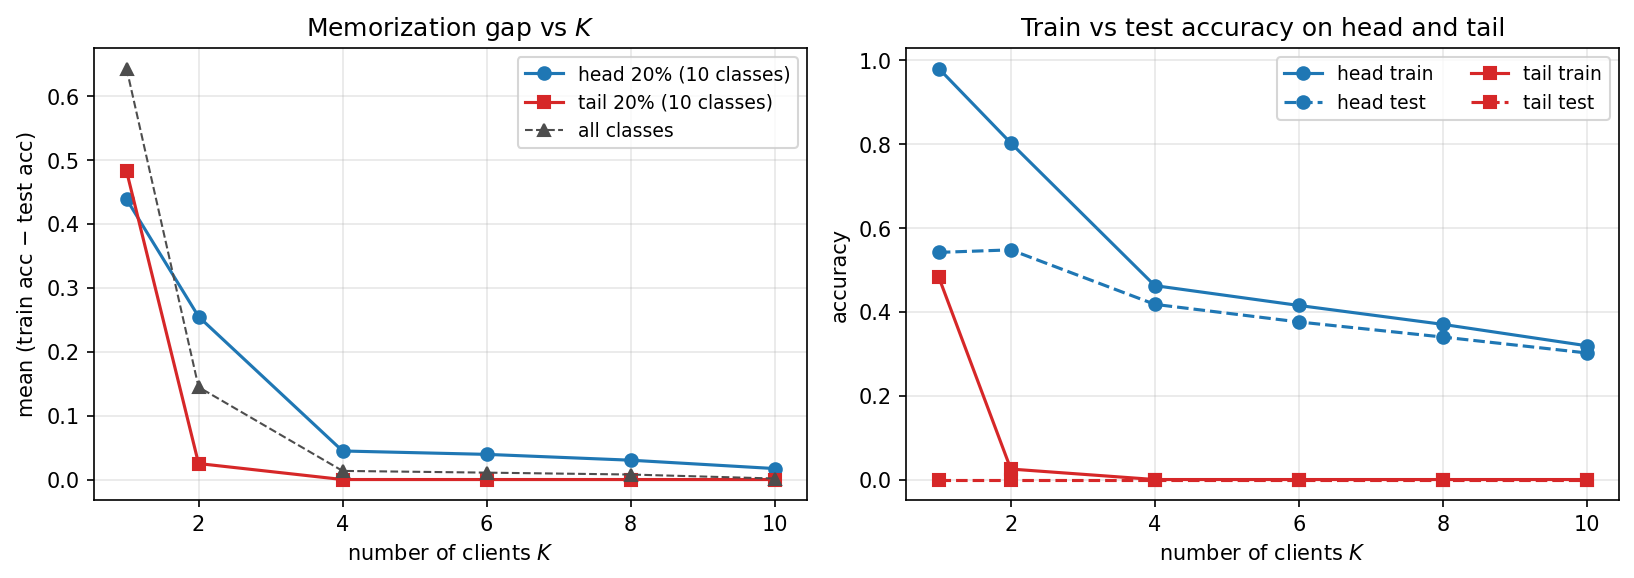
\includegraphics[width=\linewidth]{figures/fig3_summary_vs_K.png}
\caption{Community-level memorization gap as a function of the number of clients \(K\), holding the clip bound \(C=10\) and noise scale \(\sigma=3\times 10^{-4}\) fixed. \textbf{Left:} mean train--test gap on head 20\% of classes (blue), tail 20\% (red), and across all 50 classes (gray). \textbf{Right:} train (solid) versus test (dashed) accuracy on head and tail classes. The monotone collapse of the gap from \(\sim\)44 percentage points (head) and \(\sim\)48 (tail) at \(K=1\) to \(\le 1\) at \(K=10\) is consistent with the \(O(1/K^2)\) per-client memorization bound of Theorem~\ref{thm:multi-round}.}
\label{fig:summary-vs-K}
\end{figure}

\paragraph{Per-client memorization gap.} Figure~\ref{fig:per-client-box} shows the distribution across clients of per-client train accuracy, test accuracy, and train--test gap, for each \(K\). The gap distribution shrinks monotonically with \(K\): median gap drops from 75 percentage points at \(K=1\) to \(\approx 15\) at \(K=10\), with inter-client variance also tightening. At \(K=10\) every individual client has a train--test gap below 30 points, compared to gaps in excess of 70 points for the centralized run.

\begin{figure}[h]
\centering
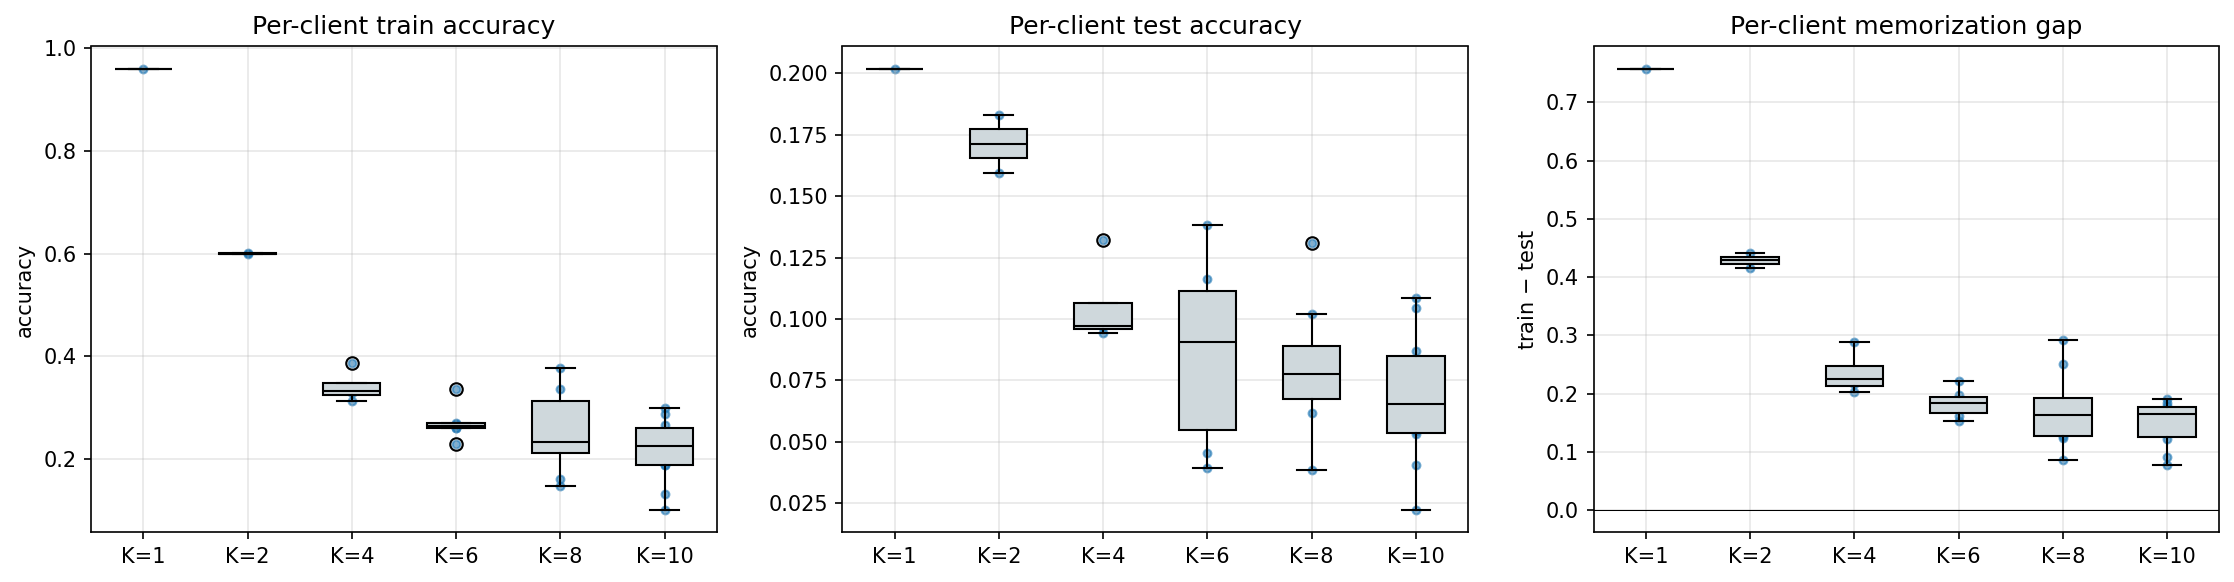
\includegraphics[width=\linewidth]{figures/fig6_per_client_box.png}
\caption{Per-client distributions of train accuracy (left), test accuracy (middle), and train--test gap (right), as a function of \(K\). Each box aggregates over the \(K\) clients in that run. The per-client gap distribution shrinks monotonically with \(K\), consistent with the per-client bound \(I(X_k;\transcript\mid P)=O(1/K^2)\).}
\label{fig:per-client-box}
\end{figure}

\paragraph{Per-class detail at \(K=10\).} Figure~\ref{fig:client-heatmap} gives a per-client per-class view at \(K=10\): one row per client, one column per class (sorted from head to tail; gray cells indicate classes the client did not own). The rightmost panel, the train--test gap, is near-uniformly white (gap close to zero) across both head and tail classes, confirming that at \(K=10\) the residual memorization signal on individual clients is essentially gone and that the residual head-class accuracy seen in Figure~\ref{fig:summary-vs-K} comes from generalizable structure, not from fitting individual rare examples.

\begin{figure}[h]
\centering
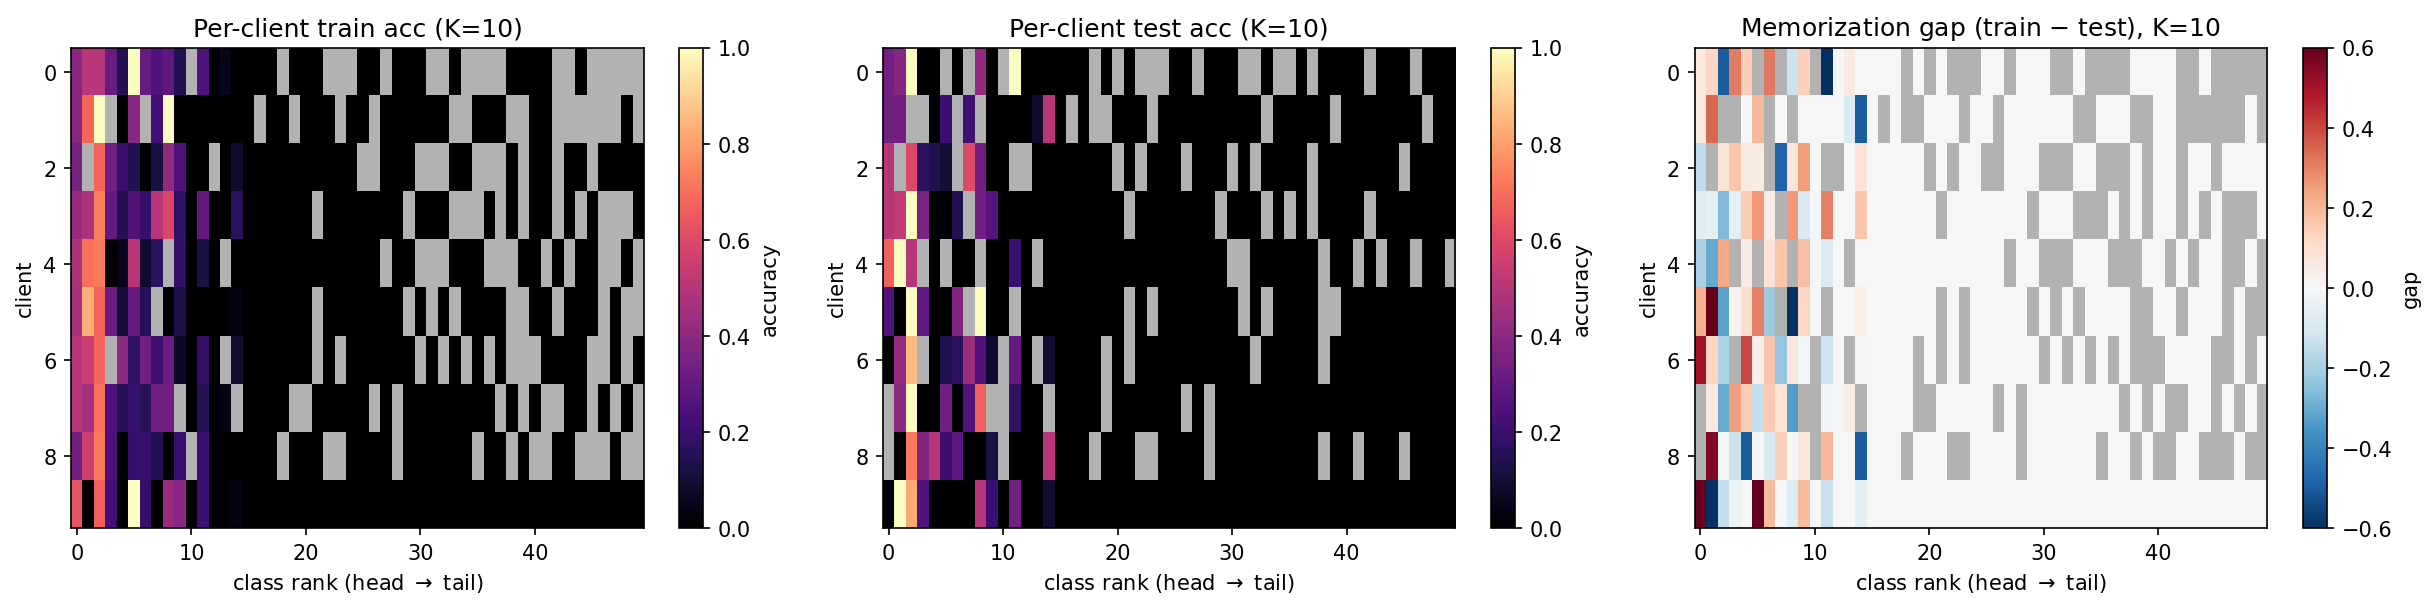
\includegraphics[width=\linewidth]{figures/fig4_client_heatmap.png}
\caption{Per-client, per-class breakdown at \(K=10\): train accuracy (left), test accuracy (middle), and train--test gap (right). Rows index clients, columns index classes (sorted head\(\to\)tail). Gray cells mark classes that a given client did not receive in its Dirichlet partition. The gap panel is near-uniformly white, indicating that the per-client memorization signal has collapsed.}
\label{fig:client-heatmap}
\end{figure}

\paragraph{Caveats.} The train--test gap is a lower-bound proxy, not a direct estimator of \(I(X_k;\transcript\mid P)\); a small empirical gap is consistent with both small CMI and with a model that has memorized but failed to retrieve at evaluation time. The experiment also operates at a noise scale (\(\sigma=3\times 10^{-4}\)) far below what a deployed DP-FedAvg system would use---this was chosen so that the centralized \(K=1\) baseline could exhibit the strong memorization predicted by \citet{Brown2021Memorization} and that our bound then collapses; the qualitative \(K\)-dependence of the gap is the comparison of interest, not the absolute privacy level. Finally, the bound concerns the transcript \(\transcript\) (or by post-processing the final iterate \(\theta^{(T)}\)); we treat the trained model's behavior on training versus test inputs as a downstream proxy.

\section{Discussion}\label{sec:discuss}

\subsection{Quantitative interpretation}
For fixed clip \(C\) and noise \(\sigma\), Theorem~\ref{thm:one-round} gives a per-client memorization that decays as \(O(1/K^2)\). On a Brown et al.\ task that requires the whole-dataset memorization \(I(X;M\mid P)=\Omega(nd)\), the average per-client memorization is \(\Omega(nd/K)\), and Theorem~\ref{thm:one-round} therefore implies
\[
\sigma^2 \;=\; \Omega\!\left(\frac{C^2}{K\cdot nd}\right)
\]
as a necessary noise scale for one-round release on such tasks. The \(T\)-round version of the same calculation gives \(T\cdot C^2/(2K^2\sigma^2)\ge \Omega(nd/K)\), i.e., \(\sigma^2 \;=\; \Omega\!\bigl(T C^2/(K\cdot nd)\bigr)\).

\subsection{Comparison: averaging vs.\ no averaging}
If each client's clipped update were instead released with independent Gaussian noise of the same scale, Lemma~\ref{lem:gauss-mi} gives \(I(X_k;U_k+Z_k\mid P)\le C^2/(2\sigma^2)\). Theorem~\ref{thm:one-round} is a factor of \(K^2\) tighter. Averaging \emph{before} adding noise at the same per-coordinate scale therefore strictly improves per-client memorization by \(K^2\). The improvement is information-theoretic; it is not a privacy-accounting artifact.

\subsection{Comparison: whole-dataset bound}
Applying Lemma~\ref{lem:gauss-mi} directly to \(S=\tfrac{1}{K}\sum_k U_k\) and using the triangle inequality \(\|S\|\le C\) gives the whole-dataset bound \(I(X;\noised\mid P)\le C^2/(2\sigma^2)\). Theorem~\ref{thm:one-round} is sharper for individual clients by a factor of \(K^2\), because each client's signal is scaled by \(1/K\) within the average even though the average's overall norm need not shrink.

\subsection{From per-client to per-record memorization}
If client \(k\)'s data is \(X_k=(X_{k,1},\dots,X_{k,n_k})\), the data-processing inequality gives
\(I(X_{k,i};M\mid P) \le I(X_k;M\mid P) \le C^2/(2K^2\sigma^2)\) (one-round) and the analogous transcript bound. Per-record memorization is therefore at most the per-client bound. The bound makes no assumption about how \(U_k\) is computed from \(X_k\), so it applies whether \(U_k\) is a one-step gradient, a multi-step local update, a model delta, or a more complex client-side optimization output.

\subsection{What this paper does not say}
We make no claim about plain (non-private) FedAvg, where the released signal is \(\Delta=\tfrac{1}{K}\sum_k U_k\) with no noise. The mutual information \(I(X_k;\Delta\mid P)\) can be \(\Omega(1)\)---or even saturate \(H(X_k\mid P)\)---without further structural assumptions, since \(\Delta\) is a deterministic function of \((X,R)\) and high-dimensional models do not offer an inherent contraction. Establishing strong data-processing-style contractions for vanilla averaging in realistic regimes is an interesting open direction.


\section*{Acknowledgments}
% Anonymized for submission.

\bibliographystyle{plainnat}
\bibliography{refs}

\end{document}
